%% 
%% Copyright 2007, 2008, 2009 Elsevier Ltd
%% 
%% This file is part of the 'Elsarticle Bundle'.
%% ---------------------------------------------
%% 
%% It may be distributed under the conditions of the LaTeX Project Public
%% License, either version 1.2 of this license or (at your option) any
%% later version.  The latest version of this license is in
%%    http://www.latex-project.org/lppl.txt
%% and version 1.2 or later is part of all distributions of LaTeX
%% version 1999/12/01 or later.
%% 
%% The list of all files belonging to the 'Elsarticle Bundle' is
%% given in the file `manifest.txt'.
%% 

%% Template article for Elsevier's document class `elsarticle'
%% with numbered style bibliographic references
%% SP 2008/03/01

\documentclass[preprint,12pt]{elsarticle}

%% Use the option review to obtain double line spacing
%% \documentclass[authoryear,preprint,review,12pt]{elsarticle}

%% Use the options 1p,twocolumn; 3p; 3p,twocolumn; 5p; or 5p,twocolumn
%% for a journal layout:
%% \documentclass[final,1p,times]{elsarticle}
%% \documentclass[final,1p,times,twocolumn]{elsarticle}
%% \documentclass[final,3p,times]{elsarticle}
%% \documentclass[final,3p,times,twocolumn]{elsarticle}
%% \documentclass[final,5p,times]{elsarticle}
%% \documentclass[final,5p,times,twocolumn]{elsarticle}

%% For including figures, graphicx.sty has been loaded in
%% elsarticle.cls. If you prefer to use the old commands
%% please give \usepackage{epsfig}

%% The amssymb package provides various useful mathematical symbols
\usepackage{amssymb}
%% The amsthm package provides extended theorem environments
\usepackage{amsthm}
%% Tthe amsmath package provides the "align" environment for nicer equation formatting
\usepackage{amsmath}
\def\bibsection{\section*{References}}
%% The lineno packages adds line numbers. Start line numbering with
%% \begin{linenumbers}, end it with \end{linenumbers}. Or switch it on
%% for the whole article with \linenumbers.
%% \usepackage{lineno}

\journal{Energy}

\begin{document}

\begin{frontmatter}

%% Title, authors and addresses

%% use the tnoteref command within \title for footnotes;
%% use the tnotetext command for theassociated footnote;
%% use the fnref command within \author or \address for footnotes;
%% use the fntext command for theassociated footnote;
%% use the corref command within \author for corresponding author footnotes;
%% use the cortext command for theassociated footnote;
%% use the ead command for the email address,
%% and the form \ead[url] for the home page:
%% \title{Title\tnoteref{label1}}
%% \tnotetext[label1]{}
%% \author{Name\corref{cor1}\fnref{label2}}
%% \ead{email address}
%% \ead[url]{home page}
%% \fntext[label2]{}
%% \cortext[cor1]{}
%% \address{Address\fnref{label3}}
%% \fntext[label3]{}

\title{Energy and exergy analysis of a cruise ship}

%% use optional labels to link authors explicitly to addresses:
%% \author[label1,label2]{}
%% \address[label1]{}
%% \address[label2]{}

\author[EPFL]{Francesco Baldi}
\author[Linneus]{Fredrik Ahlgren}
\author[DTU]{Tuong-Van Nguyen}
\author[CTU]{Cecilia Gabrielii}
\author[CTU]{Karin Andersson}

\address[EPFL]{Industrial Process Energy Systems Engineering (IPESE), \'{E}cole Polytechnique F\'{e}d\'{e}rale de Lausanne, 1950, Sion, Switzerland}
\address[Linneus]{Kalmar Maritime Academy, Linnaeus University, Kalmar, Sweden}
\address[DTU]{Department of Mechanical Engineering, Technical University of Denmark, Lyngby, Denmark}
\address[CTU]{Department of Mechanics and Maritime Sciences, Chalmers University of technology, Gothenburg, Sweden}

\begin{abstract}
%% Text of abstract

\end{abstract}

\begin{keyword}
%% keywords here, in the form: keyword \sep keyword

%% PACS codes here, in the form: \PACS code \sep code

%% MSC codes here, in the form: \MSC code \sep code
%% or \MSC[2008] code \sep code (2000 is the default)

low carbon shipping \sep energy analysis \sep exergy analysis \sep energy efficiency

\end{keyword}

\end{frontmatter}

%% \linenumbers

%% main text

%% The Appendices part is started with the command \appendix;
%% appendix sections are then done as normal sections
%% \appendix

%% \section{}
%% \label{}

%% If you have bibdatabase file and want bibtex to generate the
%% bibitems, please use
%%
%%  \bibliographystyle{elsarticle-num} 
%%  \bibliography{<your bibdatabase>}

%% else use the following coding to input the bibitems directly in the
%% TeX file.

\section{Introduction} \label{sec:introduction}

\subsection{Background}

According to the third IMO GHG Study, in 2012 CO$_2$ emissions from shipping amounted to a total of 949 million tonnes, contributing to 2.7\% of global anthropogenic CO$_2$ emissions \cite{Smith2014}. Although this contribution appears relatively low, the trend is that shipping will play an even greater role in the future due to the increased transport demand according to all IMO future scenarios \cite{Smith2014}. As an example, global transport demand has increased by 3.4\% in 2014, compared to a global GBP growth of 2.5\% the same year, which shows how shipping tends to rise even faster than global economy \cite{UNCTAD2015}.

International Energy Agency data show that the OECD countries have reduced the CO$_2$ impact from shipping, but a larger amount has been moved to the non-OECD countries [3]. The fact that shipping needs to even further reduce its CO$_2$ emissions in the near future is essential for being able to achieve the goals of maintaining the climate below a 2-degree level in 2050 [4]. Finally, in the Baltic Sea an emission control area is enforced by the International Maritime Organisation since January 2015 which stipulates that the fuel used must not contain more than 0.1\% sulphur, therefore requiring the use of more expensive distillate fuels. More generally making shipping sustainable is a challenge that will demand growing attention by the shipping industry \cite{Andersson2016}

Altogether, these conditions present a challenge to the shipping companies who attempt to reduce their fuel consumption, environmental impact, and operative costs. A wide range of fuel saving solutions for shipping are available and partially implemented in the existing fleet, both from the design and operational perspective; several specific studies have been conducted on these technologies, and a more detailed treatise would be out of the scope of this work. In this context, it has been acknowledged that the world fleet is heterogeneous, and measures need to be evaluated on a ship-to-ship basis \cite{Bouman2017}. In this process, a deeper understanding of energy use on board of the specific ship is vital.

\subsection{Previous work}

The idea of improving the understanding of the behavior of the energy system of a ship is not new. Most of the work published around this subject relates to the use  of mathematical models of the ship systems. 

Most authors focused on the propulsion part of the problem, as this is often the most relevant energy demand on board. Shi et al. proposed a modeling approach for predicting ship fuel consumption of a cargo/passenger ferry \cite{Shi2009}; Theotokoats and Tzelepis applied a similar procedure to the case of a Handymax product carrier \cite{Theotokatos2015}, similarly to Tillig et al., who also added the dynamic element to their predictive model \cite{Tillig2016}. 

The work referenced above allowed improving the understanding of how many operational (such as the ship's speed) and environmental (such as wave height and wind speed) parameters influence the ship's energy performance. These studies, however, are not based on actual measurements of the ship's operations. Also, they focus entirely on the ship's power demand for propulsion. This is a very reasonable practice for most ship types, given that propulsion represent the largest part of the total energy demand, but does not allow improving the knowledge of the remaining part of the system.

% Data-driven analysis
Other authors filled the gap by both including electric energy demand, and by basing their work on measurements from actual ship operations. The work presented by Thomas et al. \cite{Thomas2010} and Basurko et al. \cite{Basurko2013} shows the application of energy auditing methods to fishing vessels. This approach represents a step forward towards improving the understanding of how energy is used on board during actual ship operations.  

More generally, several authors have highlighted the importance of a detailed knowledge of the ship's operational profile in order to appropriately assess and optimize possible alternatives for improving ship energy efficiency \cite{Banks2013}. Coraddu et al., started from a statistical analysis of measured ship operations and used the aggregated data, together with a computational model of the vessel, to provide a better prediction of the actual ship's operational efficiency \cite{Coraddu2014}. The importance of considering the operational profile was also showed in the case of the optimization of engine-propeller interaction \cite{Baldi2015c}, in the process of retrofitting existing systems \cite{Baldi2015b,Choi2013}, and in ship design \cite{Ghassemi2017,Solem2015}. 

% Heat availability
Heat demand is rarely a subject of concern on board ships, with some notable exceptions. This is due to a combination of generally low demand and high availability from the waste heat of the engines. In a previous publications by the authors, for instance, it is shown that in the case of a product tanker, although the heat demand was estimated to account for roughly 20\% of the total energy demand of the ship on a yearly basis, it only contributes to 4.1\% of the total fuel consumption (contribution of the auxiliary boilers), while the rest of the demand is fulfilled using waste heat \cite{Baldi2015a}.

%% WHR and heat availability
It should be noted that, however, much research effort has been devoted, especially in recent times, to the improvement of the efficiency of ship energy systems by recovering the waste heat available from the engines. With reference to different types of technologies, case studies, and designs,the several authors showed the existance of a quite significant potential for energy saving when WHR systems are employed, ranging from around 1\% for single-pressure steam cycles applied to two-stroke engines \cite{Theotokatos2012} to more complex systems based on ORCs (up to 10\%, \cite{Hountalas2012}) or including the cooling systems as a source of waste heat (over10\%, \cite{Dimopoulos2012}).  The case of the installation of an ORC on board of the vessel investigated in this study (see Section \ref{sec:met:case}) was presented in \cite{Mondejar2015}, showing a similar potential.

The potential uses for waste heat on board are not limited to improving the efficiency of the power plant. Waste heat is commonly used for fulfilling on board heat demand for spatial heating and freshwater generation \cite{Molland2011,Baldi2015a,Mccarthy1990};  Balaji et al. proposed the use of waste heat for ballast-water systems \cite{Balaji2012}; Salmi et al. suggested its use for adsorption refrigeration systems \cite{Salmi2017}. A detailed review of potential uses for waste heat from marine engines is presented by Shu et al \cite{Shu2013}. 

% Cruise ships
Some ship types constitute notable examples. On cruise ships the heat demand is significantly higher compared to standard cargo ships. Referring to winter conditions, Marty et al. estimated the instantaneous heat demand of a selected cruise ship to reach roughly 23 MW, compared to an estimated peak of 49 MW for propulsion and electric auxiliaries combined \cite{Marty2012}.  


This shows how the heat from the engines should be considered as a potential resource, rather than a waste, and that there is potential for improvement based on the optimal use of these heat sources. The work presented by the authors in \cite{Baldi2016} represent a step in this direction; however, there is the need for an increased detail in the estimation of the heat demand. 

% Exergy analysis
Exergy analysis provides a more accurate estimation of the potential for energy recovery on board. The application of exergy analysis to the case of ship energy systems is, however, still limited. Dimopoulos et al. showed how the process optimizing the WHR system of a container ship can be more efficient if exergy efficiency, rather than energy efficiency, is used as the target of the optimization \cite{Dimopoulos2012}; Baldi et al. also analyzed the exergy flows on board of a product tanker, showing that this allows having a more accurate understanding of what parts of the system show potential for improvement \cite{Baldi2015a}; similar results were obtained by Marty et al., who focused on the power plant of a cruise ship \cite{Marty2016}. Koroglu et al. made a step futher also including advanced exergy analysis in their study \cite{Koroglu2017}.



\subsection{Aim}

Given the existing limitations of the current available information in scientific literature highlighted in the previous section, the objective of this work is the following:
\begin{itemize}
	\item Analyse the demand of a cruise ship in terms of propulsion power, electric power and heat, based on operational measurements.
	\item Analyse the current efficiency of the system, and potential ways to improve it, by means of applying exergy analysis
	\item Provide a more detailed analysis of the heat demand of a cruise ship, as a basis for further studies on how to optimize the whole efficiency of the propulsion plant.
\end{itemize}





\section{Method} \label{sec:method}

Here an overview of the method is provided: 
\begin{itemize}
	\item Data gathering
	\item Data filtering
	\item Data pre-processing
	\item Heat demand estimation
	\item Statistical analysis
	\item Energy and exergy analysis
\end{itemize}

In this paper, we present the application of energy and exergy analysis (described in sections \ref{set:met:energy} and \ref{sec:met:exergy} to a cruise ship. This is done for one specific case study vessel, that is described in detail in Section \ref{sec:met:case}; in Section \ref{sec:met:gathering} we present the specifics of the available information, in particular the measured data and the technical documentation; these are used to generate the required information for calculating energy and exergy flows (Section \ref{sec:met:processing}. In these regards, the estimation of the heat demand is treated in a separate section (Sec. \ref{sec:met:heat} as it constituted a particularly challenging task and it is one of the central aspects of this article. 

\subsection{Energy analysis}

\emph{Energy} can be stored, transformed from one form to another (e.g. heat to power) and transferred between systems, but can neither be created nor destroyed (conservation law)~\textbf{Bejan et al.}. The system under study is the \emph{ship energy system} and is thus taken as control volume. The energy balance can be expressed as:

\begin{align}
	\sum_{\mathrm{in}} \dot{H}_{\mathrm{in}} &= \sum_{\mathrm{out}} \dot{H}_{\mathrm{out}} \\
	\dot{H}_{\mathrm{fuel}} + \dot{H}_{\mathrm{air}} &= \sum_{{\mathrm{waste}}}\dot{H}_{{\mathrm{waste}}}+\dot{W}_{\mathrm{el}}+\dot{Q}_{\mathrm{heating}}
\end{align}

The left-hand side term represents, on a time rate basis, the energy associated with the fuel consumed in the boilers and engines ($\dot{H}_{\mathrm{fuel}}$) and the air used in the combustion processes ($\dot{H}_{\mathrm{air}}$). The right-hand side term denotes the power ($\dot{W}_{\mathrm{el}}$) and heat ($\dot{Q}_{\mathrm{heating}}$) required on-site (e.g. propulsion and fuel heating), and the heat discharged into the environment ($\sum_{{\mathrm{waste}}}\dot{H}_{{\mathrm{waste}}}$) with, for instance, the exhaust gases.

The energy flow associated with a material stream is calculated as the sum of the physical and chemical enthalpies, and kinetic and potential energies are neglected.    The physical energy is taken as the relative enthalpy, as underlined in~\textbf{Kotas et al.}, and the chemical energy is taken as the lower/higher heating value. The environmental conditions taken for the present analysis are the ambient pressure and seawater temperature.

\subsection{Exergy analysis}

\emph{Exergy} may be defined as the `maximum theoretical useful work (shaft work or electrical work) as the system is brought into complete thermodynamic equilibrium with the thermodynamic environment while the system interacts with it only'~\citep{Moran1989}. Unlike energy, exergy is not conserved but some is destroyed because of the irreversible phenomena taking place in real processes (e.g. chemical reactions like combustion). The exergy balance for the system under study can be expressed as:

\begin{align}
	\sum_{\mathrm{in}} \dot{E}_{\mathrm{in}} = \sum_{\mathrm{out}} \dot{E}_{\mathrm{out}} +\dot{E}_{d} \\
	\dot{E}_{\mathrm{fuel}} + \dot{E}_{\mathrm{air}} &= \sum_{{\mathrm{waste}}}\dot{E}_{{\mathrm{waste}}}+\dot{E}_{W}+\dot{E}_{Q,\mathrm{heating}}+\dot{E}_{d} 
\end{align}

The left-hand side term represents, on a time rate basis, the exergy associated with the fuel and air. The right-hand side term denotes the exergy of the waste streams, the exergy transfers with heat and power, and the exergy destroyed in the ship system. Kinetic and potential exergies are neglected, and the exergy of a given material stream is derived as the sum of the physical and chemical exergies. The chemical exergy is calculated based on the reference environment of \textbf{Szargut (1989)}, and its value is approximatively equal to the higher heating value for hydrocarbon fuels. The exergy destruction can be calculated from the Gouy-Stodola theorem~\textbf:{Kotas (1995)}.    

The exergy balance may alternatively be formulated as:
\begin{equation}
\dot{E}_{\mathrm{p}} = \dot{E}_{\mathrm{f}} - \dot{E}_{\mathrm{d}} - \dot{E}_{\mathrm{l}} 
\end{equation}

where $\dot{E}_{\mathrm{p}}$ is called the exergy product, and corresponds to the desired output of the system, in exergy terms (for example, the power produced in an engine). $\dot{E}_{\mathrm{f}}$ denotes the exergy fuel, and represents the resources spent to drive the studied process (for instance, the fuel used in a combustion process). The last term $\dot{E}_{\mathrm{l}}$ corresponds to the losses of a system, such as the heat discharged into the environment with cooling water. 

\subsection{System performance}

The following indicators are used to evaluate the system performance:
\begin{itemize}
	\item the exergy efficiency $\varepsilon$, defined as the ratio between the exergy product and fuel of a given component or system
	\begin{equation} \varepsilon = \frac{\dot{E}_{\mathrm{p}}}{\dot{E}_{\mathrm{f}}} \end{equation}
	\item the efficiency defect $\lambda$, presented in the work of Kotas, defined as the fraction of the total exergy input destroyed in the successive irreversible processes
	\begin{equation} \lambda = \frac{\dot{E}_{\mathrm{d}}}{\dot{E}_{\mathrm{in,tot}}} \end{equation}
	\item  the irreversibility share $\delta$, suggested in the work of Tsatsaronis, defined as the ratio between the exergy destroyed in the $i$-th component in relation to the exergy destroyed in the entire system
	\begin{equation} \delta_i = \frac{\dot{E}_{\mathrm{d},i}}{\dot{E}_{\mathrm{d,tot}}} \end{equation}
	
\end{itemize}    


\subsection{Case study vessel} \label{sec:met:case}

The energy and exergy analysis are here applied to a specific  cruise ship operating daily cruises in the Baltic Sea between Stockholm and the island of \.{A}land. The ship is 176.9 m long and has a beam of 28.6 m, and has a design speed of 21 knots. The ship was built in Aker Finnyards, Raumo Finland in 2004.

The ship has a capacity of 1800 passengers and has several restaurants, night clubs and bars, as well as saunas and pools. This means that the energy system regarding the heat and electricity demand is more complex than a regular cargo vessel in the same size. Typical ship operations, although they can vary slightly between different days, are represented in Figure \ref{fig:typicalShipOperations}. It should be noted that the ship stops and drifts in open sea during night hours before mooring at its destination in the morning, if allowed by weather conditions.

The ship systems are summarized in Figure \ref{fig:shipSystems}. The propulsion system is composed of two equal propulsion lines, each made of two engines, a gearbox, and a propeller. The main engines are four Wärtsilä 4-stroke Diesel engines (ME) rated 5850 kW each All engines are equipped with selective catalytic reactors (SCR) for NOX emissions abatement. Propulsion power is needed whenever the ship is sailing; however, it should be noted that the ship rarely sails at full speed, and most of the time it only needs one or two engines operated simultaneously.

Auxiliary power is provided by four auxiliary engines (AE) rated 2760 kW each. Auxiliary power is needed on board for a number of alternative functions, from pumps in the engine room to lights, restaurants, ventilation and entertainment for the passengers. 

Auxiliary heat needs are fulfilled by the exhaust gas steam generators (HRSG) located on all four AEs and on two of the four MEs or by oil-fired auxiliary boilers (mainly when in port, or during winter), by the heat recovery on the HT cooling water systems (HRHT), and by the auxiliary, oil fired boilers (AB). The heat is needed for passenger and crew accommodation, as well as for the heating of the highly viscous heavy fuel oil used for engines and boilers. This last part, however, is drastically reduced since the 1st of January 2015, as new regulations entering into force require the use of low-sulphur fuels, which require a much more limited heating.

\subsection{Data gathering and pre-processing} \label{sec:met:gathering}

This section should be written by FA :-)

Since measurements of ambient and seawater temperature from onboard logging systems were not available for the whole dataset, we used measurements taken from SMHI database for Landsort lighthouse. The assumption was validated based on  June-December period, for which onboard measurements were available. This resulted in a root mean square error of 1.5 K and 1.9 K for the seawater and the ambient temperature respectively, which we considered to be accurate enough for the purpose of this work.
% We did the calculation, resampling the data from SHMI from a 1(3)h to 15min frequency using linear interpolation. 

\subsection{Data processing: Ship energy system modeling} \label{sec:met:modeling}

Not all of the variables required to perform a full energy and exergy analysis of the system are available from measurements. In some cases, they are measurable, but not measured (e.g. some temperatures, mass flows, etc.). In other cases, they are simply impossible, or impractical, to measure (e.g. specific enthalpy, specific entropy). For this reason, part of the ship systems needed to be modeled in order to derive the unknown variables. 

\subsubsection*{Main engines}

Make a figure representing the main engines, with specified the variables for which we have measurements of. 

List the main assumptions

\subsubsection*{Auxiliary engines}

Make a figure representing the main engines, with specified the variables for which we have measurements of. 

List the main assumptions

\subsubsection*{Auxiliary boilers}

\subsubsection*{Cooling systems}

\subsection{Estimation of the heat demand} \label{sec:met:heat}

\subsubsection*{Production-side}

In a top-down model, the demand of an energy system is modeled based on the production side of the energy balance. According to the top-down approach, the total heat consumption is calculated based on the sum of the heat provided by the three main heat sources available on board:
\begin{itemize}
	\item Exhaust gas boilers
	\item Auxiliary oil-fired boilers
	\item Heat recovery on the HT cooling systems
\end{itemize}

For the case of the EGBs, the heat transferred from the exhaust gas to the steam ($\dot{Q}_{EGB}$) is calculated according to equation \ref{eq:egb}:
\begin{equation}
\dot{Q}_{EGB} = \dot{m}_{eg} c_{p,eg} (T_{eg,EGB,in} - T_{eg,EGB,out})
\end{equation}\label{eq:egb}

Where measurements of the exhaust gas temperature before and after the EGBs (respectively $T_{eg,EGB,in}$ and $T_{eg,EGB,out}$) are available from the DLS; the mass flow of exhaust gas ($\dot{m}_{eg}$) is calculated as described in appendices \ref{app:me} and \ref{app:ae}; and the specific heat at constant pressure of the exhaust gas ($c_{p,eg}$) is assumed to be constant and equal to 1.08 $\frac{kJ}{kgK}$.

For the case of the ABs, the heat transferred to the steam ($\dot{Q}_{AB}$) is calculated according to equation \ref{eq:ab}:
\begin{equation}
\dot{Q}_{AB} = \dot{m}_{fuel,AB} \eta_{AB}
\end{equation} \label{eq:ab}

Where the fuel consumption of the ABs ($\dot{m}_{fuel,AB}$) is available on a monthly basis. No information was available concerning the first-law efficiency of the boilers ($ \eta_{AB}$). \cite{Cohen1962} estimated it to vary between 0.83 and 0.89 depending on the load of the boiler, while according to a more recent experimental campaign presented in \cite{Mrzljak2017} the efficiency varies between 0.7 and 0.79. In the absence of more specific available data, a value of 0.8 was selected for $ \eta_{AB}$

The contribution from the heat recovery on the high temperature cooling systems of the engines ($\dot{Q}_{HRHT}$) represents the main uncertainty related to the top-down estimations. This contribution cannot be measured, neither directly or indirectly, and hence needs to be estimated. 

For this reason, two calculated values for the top-down heat demand are provided:
\begin{itemize}
	\item A \textbf{high boundary} case, where it is assumed that almost all of the heat available from the HT cooling systems (an utilization factor of 0.9 is assumed to account for losses) is used. This corresponds to the assumption that the use of the waste heat from the HT cooling systems is prioritized over the use of waste heat from the exhaust gas of the engines.
	\begin{equation}
	\dot{Q}_{HRHT} = f_{HRHT} \dot{Q}_{HT,tot} 
	\end{equation}
	\item a \textbf{low boundary} case, where it is assumed that the waste heat from the cooling systems is only used when the ship is in port (again assuming a utilization factor of 0.9). 
	\item a reference case, (NOTE: We should discuss what the assumption could be here. The one we had in the ECOS paper? Or a value halfway between the highest and lowest estimate?)
\end{itemize}

In both cases, the available heat from the HT cooling systems is estimated as explained in Section \ref{eq:met:modeling}.



\subsubsection*{Consumers-side}
Following, the assumptions that we have made related to the bottom-up estimations of ship heat demand:
\begin{itemize}
	\item In the HVAC unit, the "\textbf{Preheater}" is only used when heating (i.e., in winter) while the "\textbf{Reheater}" is only used when cooling (i.e., in summer)
	\item \textbf{Spacial heating} demand during \textbf{winter} is linearly dependent on the external air temperature, from a minimum of 0 for an external temperature of 20$^o$C to a maximum of 3500 kW (design power of the preheater)  for an outer air temperature of -20$^o$C.
	\item \textbf{Spacial heating} demand during \textbf{summer} is related to the need for dehumidification, and harder to estimate based on available measurements. As a first assumption, it is estimated to be equal to the cooling demand (estimated as detailed in Sec. ref{sec:met:electric})
	\item Every passenger contributes with a total of 150 W of free heat during the day (8-23, ref. to "walking, seated" activity from \cite{Wang2000}) and 100 W during night (23-8, ref. to "seated at rest" activity from \cite{Wang2000}). For the crew, as it is assumed that they perform a more intense activity than the passengers, the daily contribution is considered equal to 160 (ref. to "moderate work" activity from \cite{Wang2000}) 
	\item The heat required for \textbf{tank heating} is linearly dependent on the external sea water temperature. The maximum heat is required for an external seawater temperature of 0$^o$C
	\item The heat required from the \textbf{galley} depends on two parameters:
	\begin{itemize}
		\item The \textbf{number of passengers} (linear dependence)
		\item the \textbf{hour of the day}. See Figure \ref{fig:hwhvstime}
	\end{itemize}
	\item The heat required from the \textbf{hot water} depends on two parameters:
	\begin{itemize}
		\item The \textbf{number of passengers} (linear dependence)
		\item the \textbf{hour of the day}. The hour-dependent factor is assumed based on the estimations for a land-based hotel reported in \cite{Chung2015}.
	\end{itemize}   
\end{itemize}

In Table \ref{tab:heatConsumers} we summarize all heat consumers on board the case study vessel. For each entry, we provide the design heat demand and the variables we assumed the actual heat demand to depend on:
\begin{table}
	\begin{tabular}{lrccccc}
		\hline 
		Name & $\dot{Q}_{des}$ [kW] & \multicolumn{5}{c}{Depends on...} \\ 
		\hline 
		 & & $T_{air}$ & t & $N_{pax}$ & $f_{TL}$ & $\lambda$ \\ 
		\hline 
		Hot water heater & 1200 &  & x & x &  &  \\ 
		HVAC Preheater & 3500 & x & x & x &  &  \\ 
		HVAC Reheater & 1780 & x & x & x &  &  \\ 
		Tank heating & 208 &  &  &  & x &  \\ 
		Other tanks & 138 &  &  &  & x &  \\ 
		HFO Tank heating & 271 &  &  &  & x &  \\ 
		Machinery space heaters & 281 & x &  &  &  &  \\ 
		Bilge water separator & 26 &  &  &  &  &  \\ 
		Hot water calorifier & 366 &  & x &  &  &  \\ 
		Fuel oil heater & 103 &  &  &  &  & x \\ 
		HFO Separator & 37 &  &  &  &  &  \\ 
		Galley & 602 &  & x & x &  &  \\
		\hline 
	\end{tabular} \label{tab:heatConsumers}
\end{table}


\subsection{Estimation of the electric power demand} \label{sec:met:electric}

The total electric power demand of the system is easily estimated as the sum of the power generated by the four auxiliary engines, that is directly measured on the electrical side of the generators and has a rather high accuracy
\begin{equation}
P_{el,tot} = \sum_{1}^{4} AE_i
\end{equation}

The determination of how different consumers contribute to the total electric power demand is less trivial. The ship is equipped with a number of different systems, including lighting, navigational systems, pumps and compressors, etc. None of the individual contributions is directly measured, hence estimations need to be based on indirect measurements. 

\subsubsection*{HVAC systems}

For what concerns the air conditioning unit demand (HVAC), the observation of the total power demand over the year (see Figure \ref{fig:pelvstime}, showing daily averages) leads to the identification of a clear period, corresponding to the summer months, during which there is a significant increase of the demand. 

\begin{figure}
	\centering
	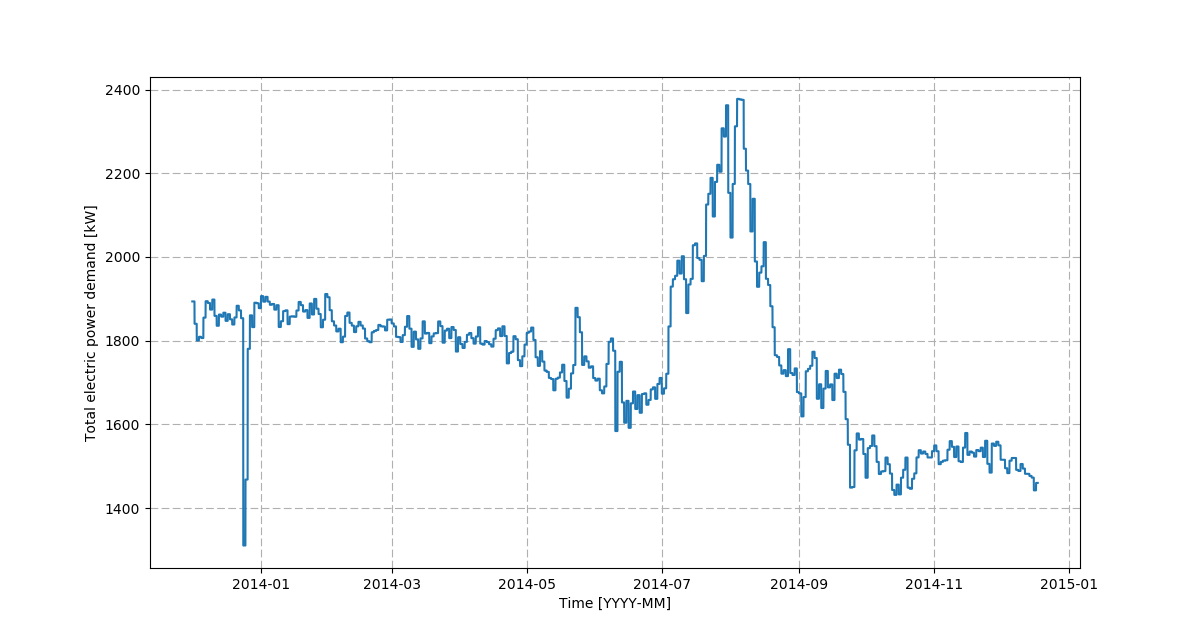
\includegraphics[width=0.9\linewidth]{Figures/Pel_vs_time}
	\caption[Total electric power demand versus time (Daily average)]{Total electric power demand versus time (Daily average)}
	\label{fig:pelvstime}
\end{figure}

Since the total demand seems to be rather constant otherwise, it can be concluded that the demand of the HVAC compressors related to the need for cooling is concentrated during the summer months. Additionally, comparing the evolution of the daily demand (see Figure \ref{fig:pelrelvstime}, representing the instantaneous demand divided by the daily average) between a random summer and winter day, shows that the daily variation is comparable. This shows that assuming a constant consumption for the HVAC during the day does not introduce a substantial error in the estimations.

\begin{figure}
	\centering
	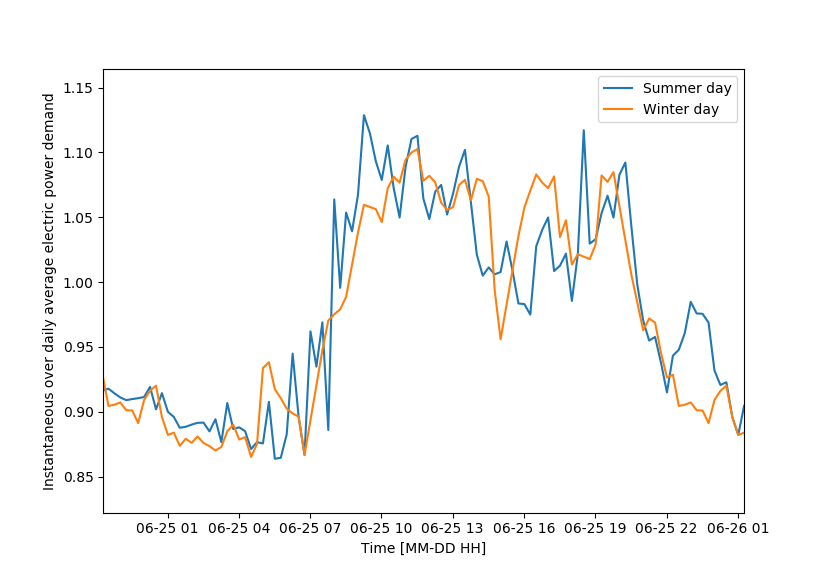
\includegraphics[width=0.9\linewidth]{Figures/PelRel_vs_time}
	\caption{Instantaneous power demand over daily average, winter versus summer day}
	\label{fig:pelrelvstime}
\end{figure}

Hence, the HVAC electric power demand was estimated as follows:
\begin{equation}
P_{el,HVAC} =
\begin{cases}
P_{el,tot}(t) - P_{el,ref}(t) , & \text{if}\ \text{2014-07-03} < t < \text{2014-08-21} \\
0, & \text{otherwise}
\end{cases}
\end{equation}
where $P_{el,ref}(t)$ is calculated as:
\begin{equation}
	P_{el,ref}(t) = 0.5 (P_{el,tot}(t_1) + P_{el,tot}(t_2))
\end{equation}


\subsubsection*{Thrusters}

When entering port areas, the ship needs to use thrusters to maneuver and berth. In the case of this particular ships, operating on daily schedules and hence maneuvering four times per day, the power demand related to thrusters can be significant. 

The observation of Figure XX shows how the power demand from thrusters can be identified as "spikes" in the total electric power demand. In order to isolate the demand from the thrusters, we created a reference daily energy profile, based on the instantaneous electric power demand divided by the daily average. From this daily profile (made of 96 points), we selected manually selected the points that could be clearly identified as related to the thrusters energy demand, and substituted the actual value with a weighted average of the previous and subsequent points (see Figure \ref{fig:thruster_selection}). 

By comparing the reference profile to the instantaneous one, the points where the former is more than 10\% higher than the latter are identified as "thruster-on" points and treated consequently. 

\begin{figure}
	\centering
	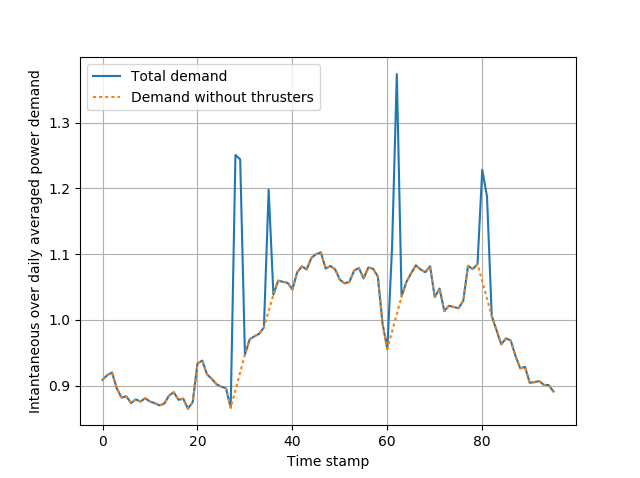
\includegraphics[width=0.9\linewidth]{Figures/Thruster_selection}
	\caption{Example of the procedure of selection of thruster power demand}
	\label{fig:thruster_selection}
\end{figure}




\section{Results (and discussion)}

\subsection{Exploratory analysis} \label{sec:res:exploratory}

In this section, we observe and analyze direct measurements from ship systems, with no pre-processing, that are expected to have an influence on the energy analysis.

Figure \ref{fig:Tsea_vs_time} represents the distribution and the evolution over the year of the ambient air and sea water temperature. The relatively low temperatures that are experienced by the case study ship during its operations suggest that heating demand can be expected to be higher than cooling demand. On the other hand, the fact that, in summer, air temperatures reach up to 26 degrees Celsius justify the existence of an HVAC unit that can also operate in cooling mode. 

The corresponding ditributions are presented in Figure \ref{fig:Tsea_hist}

\begin{figure}
	\centering
	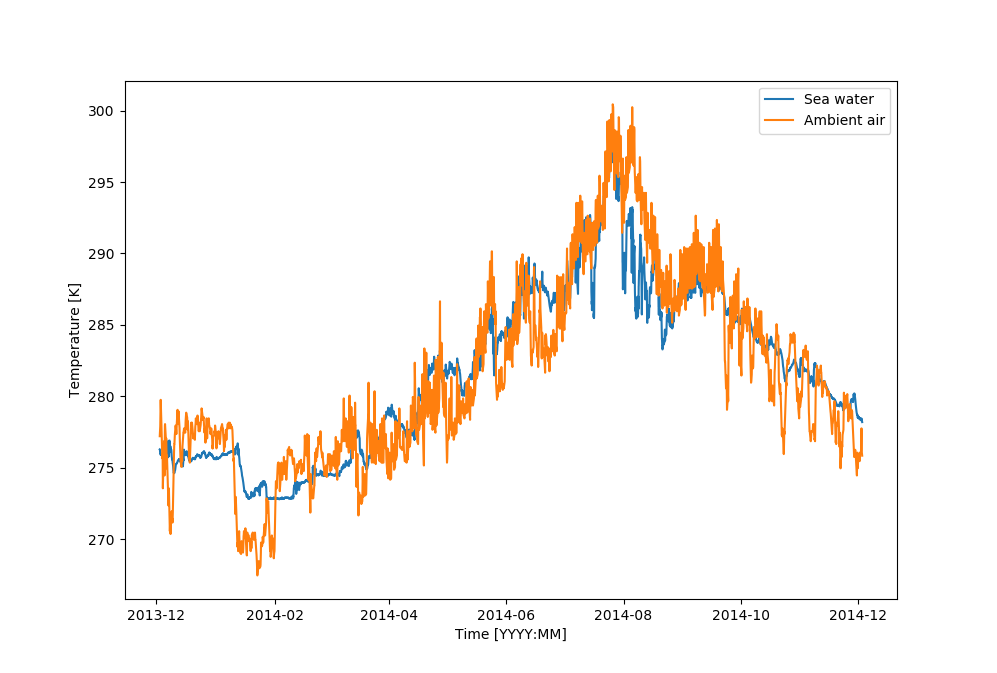
\includegraphics[width=0.9\linewidth]{Figures/Tsea_vs_time}
	\caption{Yearly evolution of sea water and ambient air temperatures. Landsort, 2014}
	\label{fig:Tsea_vs_time}
\end{figure}

\begin{figure}
	\centering
	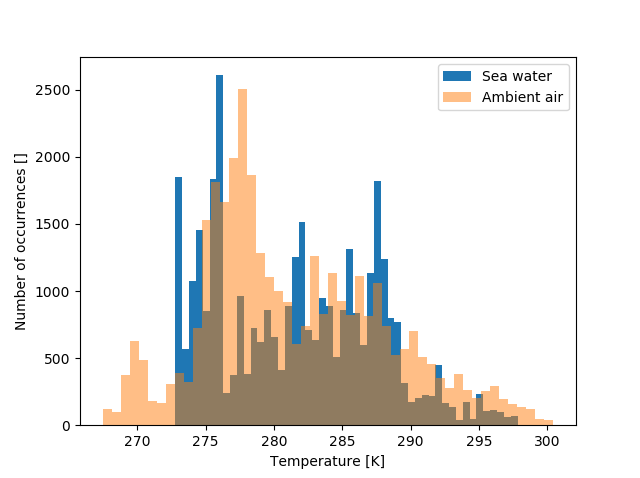
\includegraphics[width=0.9\linewidth]{Figures/Tsea_hist}
	\caption{Yearly distribution of sea water and ambient air temperatures. Landsort, 2014}
	\label{fig:Tsea_hist}
\end{figure}

Figure \ref{fig:vship_hist} represents the distribution of the ship speed, both in terms of statistical distribution and in terms of a reference 24h period. The ship operates almost for the entire year according to a fix schedule. 

NOTE: It would be interesting to find a way to categorize all periods in each phase (sailing in the archipelago - sailing at open sea) and trying to analyze statistically their duration / mean power / etc.

\begin{figure}
	\centering
	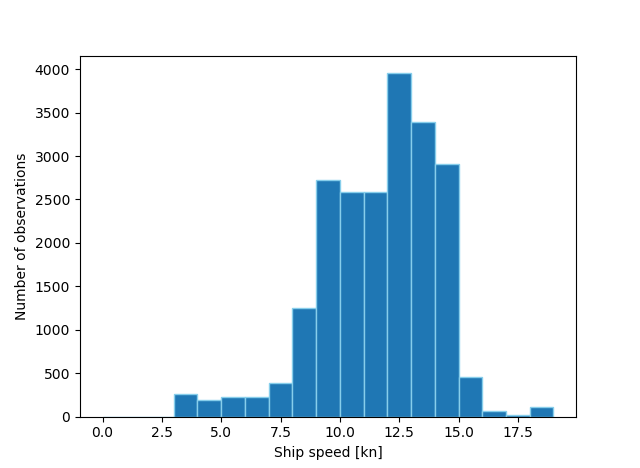
\includegraphics[width=0.9\linewidth]{Figures/vship_hist}
	\caption{Yearly distribution of ship speed}
	\label{fig:vship_hist}
\end{figure}

\begin{itemize}
	\item External temperature
	\item Sea water temperature
	\item Ship speed
\end{itemize}

The results are presented in two main forms:
\begin{itemize}
	\item Time series (comparing some relevant trips with a daily time scale)
	\item Distribution plot (or box plot...box plots are easier to compare, distribution plots are easier to interpret)
\end{itemize}

\subsection{Energy analysis} \label{sec:res:energy}

The results are presented in three main forms:
\begin{itemize}
	\item Time series (comparing some relevant trips with a daily time scale)
	\item Distribution plot (or box plot...box plots are easier to compare, distribution plots are easier to interpret)
	\item Sankey diagrams
\end{itemize}

The results should be presented both for the full database and for each operational mode (port-sailing-drifting)

\subsection{Heat demand} \label{sec:res:heat}

In Figure \ref{fig:Heat_vs_time} the heat generated by different hot utilities, as estimated by the model, is shown. It should be noticed that, while the heat generated by the HRSGs represents a rather accurate estimation, all other data series (auxiliary boilers, HTHR) are the consequence of rather strong assumptions. 

The figure also shows the operation of validation of the assumptions by comparison of the measured values for the boilers fuel consumption (here translated into an energy-per-day basis to ease the comparison). It should be noted that, although the absolute value is still quite different compared to the calculated one (mean error is 255\%, minimum 3\%), there is evidence that the order of magnitude is similar, and that some trends are followed

\begin{figure}
	\centering
	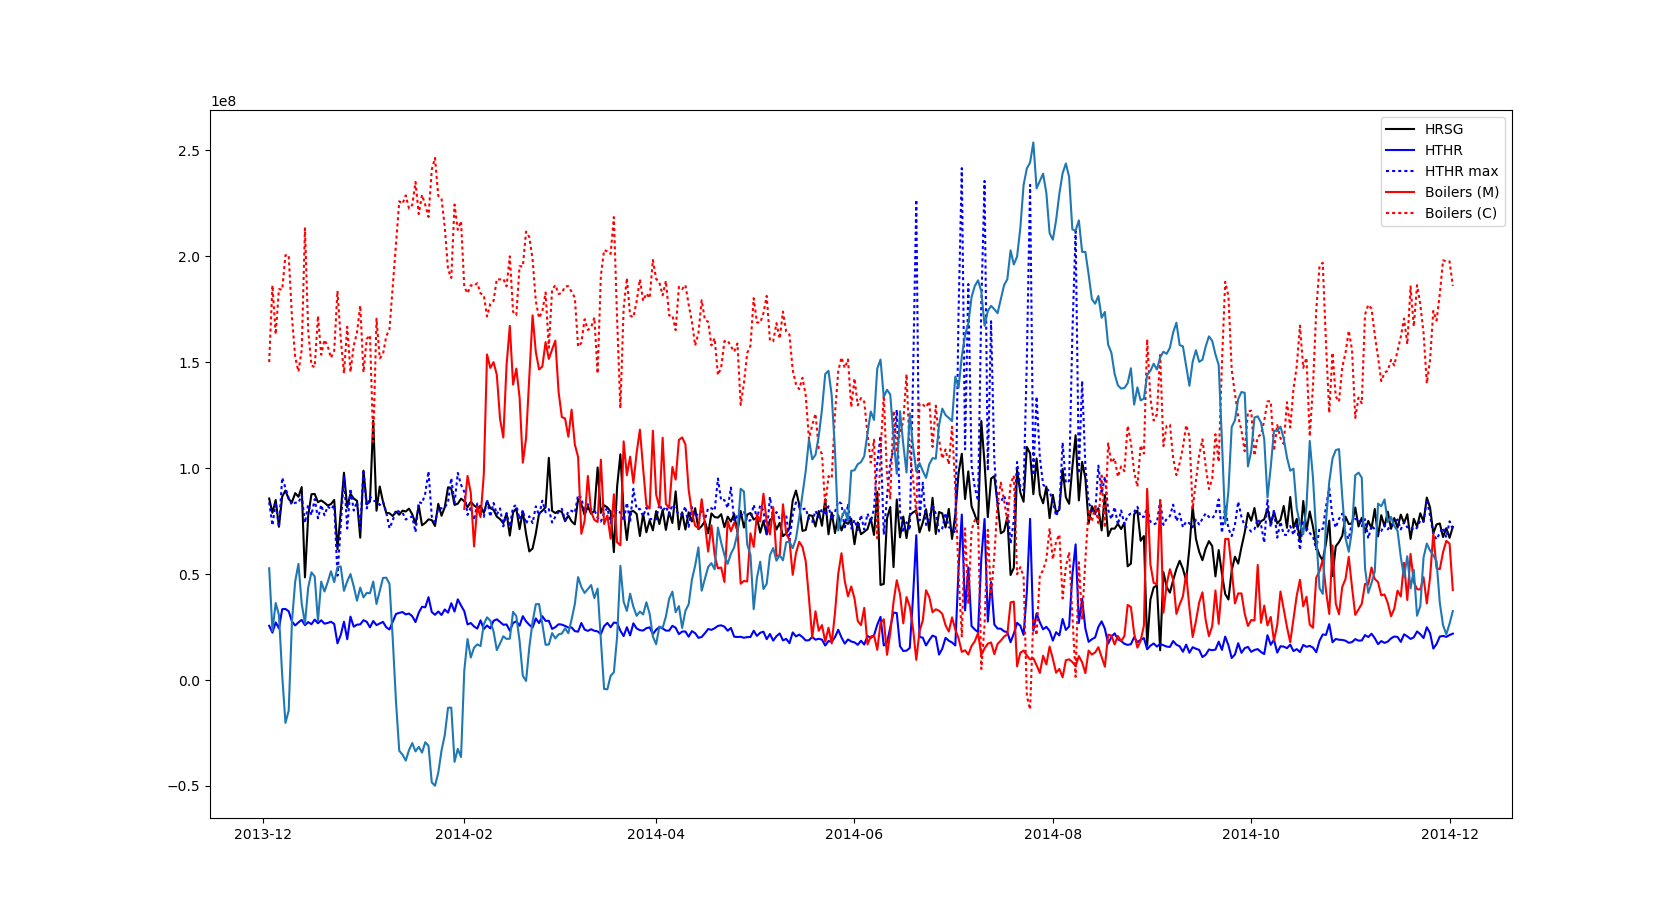
\includegraphics[width=0.99\linewidth]{Figures/Heat_vs_time}
	\caption{Yearly evolution of heat generated by different sources. "Measured" and "Calculated" relate to the auxiliary oil-fired boilers}
	\label{fig:Heat_vs_time}
\end{figure}

Estimated heat demand
Maximum heat demand 
Minimum heat demand

\subsection{Exergy Analysis} \label{sec:res:exergy}





\section{Discussion}
\label{sec:discussion}


\section{Conclusion}
\label{sec:conclusion}

\appendix

\section{Estimation of air and exhaust gas flows in the main engines}

\section{Estimation of air and exhaust gas flows in the auxiliary engines}

\bibliographystyle{unsrt}
\bibliography{bibliography}

%% \begin{thebibliography}{widestlabel}
%% \bibitem{label}
%% Text of bibliographic item
%%\end{thebibliography}

\end{document}
\endinput
%%
%% End of file `elsarticle-template-num.tex'.